\documentclass[a4paper,12pt]{report}
\usepackage{amssymb}

\usepackage{ucs}
\usepackage[utf8x]{inputenc} % Input encoding for Greek characters
\usepackage[greek,english]{babel} % Language support

\newcommand{\en}{\selectlanguage{english}}
\newcommand{\gr}{\selectlanguage{greek}}

% \usepackage{algorithm2e}
% \usepackage{algorithm}
% \usepackage{algorithmic}
\usepackage{enumitem}
\usepackage{tcolorbox}
\tcbuselibrary{listingsutf8}
\usepackage{float}
\usepackage{amsmath}
\usepackage{graphicx} % For including images
\usepackage{titlesec} % Custom title formatting
\usepackage{fancyhdr} % For custom headers and footers
\usepackage{geometry} % For adjusting page margins

% Adjust the page margins to make content wider
\geometry{top=2.5cm, bottom=2.5cm, left=2.5cm, right=2.5cm}

% Redefine chapter formatting to make it smaller
\titleformat{\chapter}[display]
    {\normalfont\LARGE\bfseries} % Smaller size and bold for chapter heading
    {\chaptername\ \thechapter} % Chapter number format
    {15pt} % Space between chapter number and title
    {\bfseries} % Smaller size and bold for chapter title
\begin{document}

\begin{titlepage}
    \centering
    \vspace*{-3cm}
    % University logo
    \includegraphics[width=1\textwidth]{auth_logo.png} % Replace with your actual logo file

    % University name in Greek
    \textbf{\gr ΑΡΙΣΤΟΤΕΛΕΙΟ ΠΑΝΕΠΙΣΤΗΜΙΟ ΘΕΣΣΑΛΟΝΙΚΗΣ}
    \vspace{2cm}

    % Document title and subtitle in Greek
    \LARGE\textbf{\gr Γραφική με Υπολογιστές Αναφορά} \\
    \Large\normalfont{\gr Εργασία 1} \\
    \vspace{4cm}

    \gr
    \large
    \textbf{Διακολουκάς Δημήτριος} \\
    \textbf{AEM 10642}
    \vspace{2.5cm}

    \en
    \textit{Email: ddiakolou@ece.auth.gr}
\end{titlepage}

\gr
\tableofcontents

\chapter{Περιγραφή Προβλήματος και Βοηθητικές Συναρτήσεις}

Η παρούσα εργασία έχει ως στόχο την υλοποίηση μεθόδων για την απόδοση χρώματος \en (shading) \gr σε τριγωνικά πλέγματα που προβάλλονται από έναν \en 3D \gr χώρο σε δισδιάστατο \en (2D) \gr καμβά.

\vspace{0.3cm}

\hspace{-0.6cm}Το αρχείο εισόδου \en \texttt{hw1.npy} \gr περιέχει δεδομένα για τις κορυφές \en (vertices)\gr, τα χρώματα \en (vcolors)\gr, τους δείκτες θέσεων τριγώνων \en (faces \gr ή \en \texttt{t\_pos\_idx})\gr, τις τιμές βάθους \en (depth) \gr και τις συντεταγμένες υφής \en (UV coordinates)\gr. Τα δεδομένα αυτά αξιοποιούνται από τη συνάρτηση \en \texttt{render\_img} \gr για να αποδοθεί η τελική εικόνα.

\vspace{0.3cm}

\hspace{-0.6cm}Ο καμβάς στον οποίο γίνεται η σχεδίαση είναι διαστάσεων $M \times N = 512 \times 512$ και έχει λευκό υπόβαθρο. Κάθε τρίγωνο σχεδιάζεται σε σειρά, ξεκινώντας από το πιο μακρινό (μεγαλύτερη τιμή \en \texttt{depth}\gr) προς το πιο κοντινό.

\vspace{0.5cm}
\noindent\textbf{Σκοπός:} Να χρωματιστούν $K$ τρίγωνα (από τον πίνακα \en \texttt{faces}\gr) με βάση δύο διαφορετικές μεθόδους:
\begin{itemize}
    \item \textbf{\en Flat shading:\gr} Κάθε τρίγωνο χρωματίζεται με το μέσο όρο των χρωμάτων των κορυφών του.
    \item \textbf{\en Texture shading:\gr} Χρήση εικόνας υφής \en (\texttt{textImg}) \gr με παρεμβολή \en UV \gr συντεταγμένων.
\end{itemize}

\section*{Βοηθητική Συνάρτηση \en \texttt{vector\_interp}\gr}

Για τις ανάγκες της παρεμβολής τιμών κατά μήκος ευθύγραμμων τμημάτων (π.χ., για υπολογισμό \en UV \gr συντεταγμένων ή \en RGB \gr χρωμάτων), χρησιμοποιούμε τη βοηθητική συνάρτηση \en \texttt{vector\_interp}\gr.
Έστω δύο σημεία $p_1 = (x_1, y_1)$ και $p_2 = (x_2, y_2)$, με αντίστοιχα διανύσματα $V_1$ και $V_2$ (π.χ. $V_1, V_2 \in \mathbb{R}^3$ για \en RGB \gr ή $V_1, V_2 \in \mathbb{R}^2$ για \en UV\gr).

\hspace{-0.6cm}Θεωρούμε ένα ενδιάμεσο σημείο $p = (x, y)$ που βρίσκεται πάνω στο ευθύγραμμο τμήμα $p_1 p_2$. Αν θέλουμε να υπολογίσουμε τη διανυσματική τιμή $V$ στο σημείο $p$ μέσω παρεμβολής στον άξονα $x$ ή $y$, τότε:

\[
t = \frac{c - c_1}{c_2 - c_1}
\]

\[
V = (1 - t) \cdot V_1 + t \cdot V_2
\]

όπου:

\begin{itemize}
    \item $c$ είναι η τετμημένη $x$ ή τεταγμένη $y$ του σημείου $p$
    \item $c_1, c_2$ είναι οι αντίστοιχες συντεταγμένες των $p_1$ και $p_2$
    \item $t \in [0, 1]$ είναι ο παράγοντας παρεμβολής
    \item $V$ είναι το διάνυσμα που προκύπτει στην ενδιάμεση θέση $p$
\end{itemize}

\hspace{-0.6cm}Αυτός ο τύπος χρησιμοποιείται εκτενώς για τον υπολογισμό ενδιάμεσων χρωμάτων και \en UV \gr συντεταγμένων κατά τον χρωματισμό \en (shading) \gr ενός τριγώνου και υλοποιείται στο αρχείο \en \texttt{vector\_interp}\gr. Είναι βασική για το \en \texttt{texture shading}\gr, καθώς χρησιμοποιείται για την παρεμβολή \en UV \gr συντεταγμένων σε κάθε \en scanline \gr και σημείο του τριγώνου.


\chapter{Διαδικασία Χρωματισμού Τριγώνων και Ψευδοκώδικας}

Σε αυτή την εργασία, εφαρμόστηκαν δύο διαφορετικές τεχνικές για τον χρωματισμό των τριγώνων που σχηματίζουν την προβολή ενός \en 3D \gr αντικειμένου στον δισδιάστατο  καμβά \en (2D canvas)\gr. Οι τεχνικές αυτές είναι οι εξής:

\begin{itemize}
    \item \en Flat Shading \gr που είναι απλός, ομοιόμορφος χρωματισμός με βάση το μέσο όρο χρωμάτων των κορυφών κάθε τριγώνου.
    \item \en Texture Mapping \gr που είναι για  χαρτογράφηση υφής με χρήση $UV$ συντεταγμένων που επιτρέπουν την απεικόνιση μιας εικόνας υφής πάνω στο γεωμετρικό πλέγμα.
\end{itemize}

\hspace{-0.6cm}Και στις δύο περιπτώσεις, ο αλγόριθμος διασχίζει κάθε τρίγωνο ξεχωριστά, και με βάση τη μέθοδο που έχει επιλεχθεί, χρωματίζει τα εσωτερικά του σημεία.

\section{\en Flat Shading\gr}

Η τεχνική \en flat shading \gr βασίζεται στον απλό και γρήγορο υπολογισμό του χρώματος κάθε τριγώνου. Το τελικό χρώμα του τριγώνου προκύπτει από το διανυσματικό μέσο όρο των χρωμάτων των τριών κορυφών του. Έπειτα, όλα τα pixels που εμπίπτουν εντός του τριγώνου βάφονται με αυτό το ενιαίο χρώμα.

\subsection*{Διαδικασία υλοποίησης}

\begin{enumerate}
    \item Για κάθε τρίγωνο, προσδιορίζεται το ελάχιστο παραλληλόγραμμο \en (bounding box)\gr που το περικλείει.
    \item Για κάθε εσωτερικό \en pixel \gr εντός του \en bounding box\gr:
        \begin{itemize}
            \item Υπολογίζεται αν το pixel ανήκει στο τρίγωνο με χρήση της \en edge function\gr, η οποία βασίζεται σε εσωτερικά γινόμενα.
            \item Αν το pixel βρίσκεται εντός του τριγώνου, τότε αποδίδεται σε αυτό το \textit{μέσο χρώμα} των κορυφών.
        \end{itemize}
\end{enumerate}

\subsection*{Ψευδοκώδικας}
\en 
\begin{tcolorbox}[colback=gray!5!white, colframe=black!75!black, title=Flat Shading Pseudocode]
\begin{verbatim}
flat_color = mean([vcolor0, vcolor1, vcolor2])

for j in range(min_y, max_y):
    for i in range(min_x, max_x):
        if point_in_triangle((i + 0.5, j + 0.5)):
            img[j, i] = flat_color
\end{verbatim}
\end{tcolorbox}
\gr

\vspace{0.3cm}

\hspace{-0.6cm}Η πλήρης υλοποίηση αυτής της τεχνικής βρίσκεται στο αρχείο \en \texttt{flat\_shading.py} \gr και ειδικότερα στη συνάρτηση \en \texttt{f\_shading}\gr, η οποία καλείται για κάθε τρίγωνο μέσα από τη \en render\_img\gr.

\section{\en Texture Shading (UV Mapping)\gr}

Η τεχνική \en texture mapping \gr προσφέρει πιο ρεαλιστικό αποτέλεσμα, καθώς επιτρέπει σε κάθε τρίγωνο να «προβάλλει» μια περιοχή της εικόνας υφής πάνω του, με βάση τις $UV$ συντεταγμένες των κορυφών του. Η μέθοδος αυτή χρησιμοποιεί την βοηθητική συνάρτηση \en \texttt{vector\_interp} \gr για γραμμική παρεμβολή.

\subsection*{Διαδικασία υλοποίησης}

\begin{enumerate}
    \item Ταξινομούνται οι κορυφές του τριγώνου κατά αύξουσα σειρά ως προς τον άξονα $y$.
    \item Για κάθε \en scanline \gr $y$ (δηλ. οριζόντια γραμμή):
        \begin{itemize}
            \item Υπολογίζονται τα σημεία τομής $A$ και $B$ στα δύο άκρα του τριγώνου (αριστερό και δεξί), χρησιμοποιώντας την \en \texttt{vector\_interp} \gr ώστε να εντοπιστούν τα $UV$ των σημείων αυτών.
            \item Εντός του διαστήματος $[A_x, B_x]$, γίνεται νέα παρεμβολή των $UV$ για κάθε $x$ και εξάγεται το κατάλληλο χρώμα από την εικόνα υφής.
        \end{itemize}
    \item Κάθε \en pixel \gr $(x, y)$ βάφεται με βάση το χρώμα που εντοπίζεται στην υφή στις συντεταγμένες $UV$.
\end{enumerate}

\begin{figure}[H]
    \centering
    \includegraphics[width=0.55\textwidth]{COLOR.png}
    \caption{Παράδειγμα γραμμικής παρεμβολής κατά το \en \texttt{Texture Mapping}\gr. Το σημείο $P=(x, y)$ αποκτά το χρώμα του μέσω παρεμβολής των $UV$ συντεταγμένων στα σημεία $A$ και $B$, τα οποία προκύπτουν με παρεμβολή πάνω στις ακμές του τριγώνου. 'Ετσι γίνεται και η βασική υλοποίηση στον κώδικα}
    \label{fig:texture_interp}
\end{figure}

\subsection*{Ψευδοκώδικας}
\en 
\begin{tcolorbox}[colback=gray!5!white, colframe=black!75!black, title=Texture Shading Pseudocode]
\begin{verbatim}
for y in min_y to max_y:
    if y < v1.y:
        A = vector_interp(v0, v1, v0, v1, y, dim=2)
        uv_A = vector_interp(v0, v1, uv0, uv1, y, dim=2)
    else:
        A = vector_interp(v1, v2, v1, v2, y, dim=2)
        uv_A = vector_interp(v1, v2, uv1, uv2, y, dim=2)

    B = vector_interp(v0, v2, v0, v2, y, dim=2)
    uv_B = vector_interp(v0, v2, uv0, uv2, y, dim=2)

    for x in ceil(A.x) to floor(B.x):
        uv_P = vector_interp(A, B, uv_A, uv_B, x, dim=1)
        color = texture_img[uv_P]
        img[y, x] = color
\end{verbatim}
\end{tcolorbox}
\gr

\vspace{0.3cm}
\hspace{-0.6cm}Η τεχνική αυτή υλοποιείται πλήρως στο αρχείο \en \texttt{texture\_shading.py} \gr και στη συνάρτηση \en \texttt{t\_shading}\gr. Η χρήση της παρεμβολής επιτρέπει την απόδοση ρεαλιστικών λεπτομερειών της υφής πάνω στην επιφάνεια του τριγώνου.


\chapter{Υλοποίηση και Κλήση Προγραμμάτων}

Σε αυτό το κεφάλαιο περιγράφεται η γενική δομή και ο τρόπος εκτέλεσης των προγραμμάτων που υλοποιήθηκαν για τις τεχνικές \en Flat Shading \gr και \en Texture Shading\gr. Η συνολική ροή περιλαμβάνει την ανάγνωση των δεδομένων, την επιλογή τεχνικής απόδοσης και την αποτύπωση του τελικού αποτελέσματος στον καμβά.

\section{Δομή Αρχείων και Κώδικα}
Η εφαρμογή αποτελείται από τα παρακάτω κύρια αρχεία:

\begin{itemize}
    \item \en \texttt{flat\_shading.py}\gr – Υλοποιεί την τεχνική \en Flat Shading\gr.
    \item \en \texttt{texture\_shading.py}\gr – Υλοποιεί την τεχνική \en Texture Shading\gr.
    \item \en \texttt{vector\_interp.py}\gr - Περιέχει τη βοηθητική συνάρτηση γραμμικής παρεμβολής \en \texttt{vector\_interp}\gr.
    \item \en \texttt{render\_utils.py}\gr – Περιέχει τη συνάρτηση \en \texttt{render\_img} \gr η οποία οργανώνει τη διαδικασία χρωματισμού.
    \item \en \texttt{demo\_f.py}\gr – Κύριο πρόγραμμα εκτέλεσης για τεχνική \en Flat Shading\gr.
    \item \en \texttt{demo\_g.py}\gr – Κύριο πρόγραμμα εκτέλεσης για τεχνική \en Texture Shading\gr.
\end{itemize}

\section{Συνάρτηση \en \texttt{render\_img}\gr}

Η \en \texttt{render\_img()}\gr είναι η βασική συνάρτηση απόδοσης. Αναλαμβάνει την προετοιμασία του καμβά, την ταξινόμηση των τριγώνων βάσει βάθους (για ορθό χειρισμό επικάλυψης) και την κλήση της κατάλληλης μεθόδου χρωματισμού για κάθε τρίγωνο.

\subsection*{Περιγραφή Λειτουργίας}

\begin{itemize}
    \item Δημιουργεί εικόνα $512 \times 512$ με λευκό φόντο.
    \item Υπολογίζει το μέσο βάθος κάθε τριγώνου με χρήση του πίνακα \en \texttt{depth}\gr.
    \item Ταξινομεί τα τρίγωνα σε σειρά από το πιο μακρινό στο πιο κοντινό.
    \item Για κάθε τρίγωνο:
    \begin{itemize}
        \item Αν η τεχνική είναι \en \texttt{flat}\gr, καλείται η \en \texttt{f\_shading()}\gr.
        \item Αν η τεχνική είναι \en \texttt{texture}\gr, καλείται η \en \texttt{t\_shading()}\gr.
    \end{itemize}
    \item Επιστρέφει την τελική εικόνα.
\end{itemize}

\subsection*{Ψευδοκώδικας}
\en
\begin{tcolorbox}[colback=gray!5!white, colframe=black!75!black, title=render\_img() Pseudocode]
\begin{verbatim}
function render_img(faces,vertices,vcolors,uvs,depth,shading,texImg):

    img = create_white_canvas(512, 512)
    triangle_depths = mean(depth[faces], axis=1)
    sorted_indices = sort_descending(triangle_depths)

    for i in sorted_indices:
        face = faces[i]
        triangle_vertices = vertices[face]

        if shading == 'f':
            triangle_colors = vcolors[face]
            img = f_shading(img,triangle_vertices,triangle_colors)

        else if shading == 't':
            triangle_uv = uvs[face]
            img = t_shading(img,triangle_vertices,triangle_uv,texImg)

    return img
\end{verbatim}
\end{tcolorbox}
\gr

\section{Τρόπος Κλήσης Προγραμμάτων}

Υπάρχουν δύο κύρια εκτελέσιμα προγράμματα:

\subsection*{1. \en Flat Shading: \texttt{demo\_f.py}\gr}

\begin{itemize}
    \item Χρησιμοποιεί την τεχνική \en \texttt{f\_shading}\gr.
    \item Δεν χρησιμοποιεί $UV$ συντεταγμένες ή εικόνα υφής.
    \item Το αποτέλεσμα αποθηκεύεται ως \en \texttt{flat\_result.png}\gr.
\end{itemize}

\hspace{-0.6cm}\textbf{Εκτέλεση:}
\en
\begin{verbatim}
python demo_f.py
\end{verbatim}
\gr
\subsection*{2. \en Texture Shading: \texttt{demo\_g.py}}

\begin{itemize}
    \item Χρησιμοποιεί την τεχνική \en \texttt{t\_shading}\gr.
    \item Φορτώνει εικόνα υφής με χρήση της \en \texttt{load\_png\_image()}\gr.
    \item Το αποτέλεσμα αποθηκεύεται ως \en \texttt{texture\_result.png}\gr.
\end{itemize}

\hspace{-0.6cm}\textbf{Εκτέλεση:}
\en 
\begin{verbatim}
python demo_g.py
\end{verbatim}
\gr 

\section{Ροή Δεδομένων}

Η συνολική ροή των δεδομένων έχει ως εξής:

\begin{center}
\en 
\texttt{hw1.npy} $\rightarrow$ \texttt{main()} $\rightarrow$ \texttt{render\_img()} $\rightarrow$ \texttt{f\_shading / t\_shading} $\rightarrow$ \gr Τελική εικόνα
\end{center}

Τα δεδομένα περιλαμβάνουν:
\begin{itemize}
    \item $L \times 2$ πίνακα κορυφών (\en \texttt{v\_pos2d}\gr)
    \item $L \times 3$ πίνακα χρωμάτων (\en \texttt{v\_clr}\gr)
    \item $L \times 1$ πίνακα βάθους (\en \texttt{depth}\gr)
    \item $L \times 2$ πίνακα $UV$ συντεταγμένων (\en \texttt{v\_uvs}\gr)
    \item $K \times 3$ πίνακα συνδεσιμότητας (\en \texttt{t\_pos\_idx}\gr)
\end{itemize}

\section{Αποτελέσματα}

Κάθε demo παράγει εικόνα με τις ακόλουθες ιδιότητες:

\begin{itemize}
    \item Διαστάσεις: $512 \times 512 \times 3$
    \item Αρχικά λευκός καμβάς
    \item Εμφανίζει το αντικείμενο ως ένωση χρωματισμένων τριγώνων
    \item Αποθηκεύεται τοπικά σε μορφή \en \texttt{PNG}\gr
\end{itemize}


\chapter{Αποτελέσματα, Οπτικοποίηση, Παρατηρήσεις}

Σε αυτό το κεφάλαιο παρουσιάζονται τα παραγόμενα αποτελέσματα από τις τεχνικές \en Flat Shading \gr και \en Texture Mapping \gr που υλοποιήθηκαν στα αντίστοιχα προγράμματα. Για λόγους σύγκρισης και κατανόησης των διαφορών, παρατίθενται τόσο οι τελικές εικόνες όσο και η εικόνα υφής που χρησιμοποιήθηκε στην τεχνική χαρτογράφησης υφής.

\section{Περιγραφή Εισόδου – Αρχείο \en \texttt{hw1.npy}\gr}

Το αρχείο \en \texttt{hw1.npy}\gr περιέχει όλα τα απαραίτητα δεδομένα για την απόδοση της προβολής ενός \en 3D \gr αντικειμένου στον δισδιάστατο καμβά. Πρόκειται για ένα \en \texttt{Python dictionary} \gr που περιλαμβάνει τις εξής δομές δεδομένων:

\begin{itemize}
    \item \en \textbf{\texttt{v\_pos2d}}\gr: \en NumPy array \gr διαστάσεων $(9641, 2)$. Περιέχει τις δισδιάστατες συντεταγμένες των κορυφών του αντικειμένου μετά την προβολή τους στον καμβά (σε \en pixels\gr).
    
    \item \en \textbf{\texttt{v\_uvs}}\gr: \en NumPy array \gr διαστάσεων $(9641, 2)$. Περιέχει τις κανονικοποιημένες $UV$ συντεταγμένες για κάθε κορυφή, οι οποίες χρησιμοποιούνται για τη χαρτογράφηση υφής.
    
    \item \en \textbf{\texttt{v\_clr}}\gr: \en NumPy array \gr διαστάσεων $(9641, 3)$. Περιέχει τις χρωματικές τιμές \en (RGB) \gr των κορυφών, με τιμές στο διάστημα $[0, 1]$.
    
    \item \en \textbf{\texttt{t\_pos\_idx}}\gr: Πίνακας τύπου \en \texttt{TrackedArray} \gr (από το \en \texttt{trimesh}\gr) διαστάσεων $(7504, 3)$. Κάθε γραμμή του πίνακα περιέχει τρεις δείκτες προς τις κορυφές που σχηματίζουν ένα τρίγωνο.
    
    \item \en \textbf{\texttt{depth}}\gr: \en NumPy array \gr διαστάσεων $(9641,)$. Περιέχει την τιμή βάθους (βάσει προβολής) κάθε κορυφής στο αρχικό τρισδιάστατο μοντέλο. Το βάθος χρησιμοποιείται για τον σωστό χρωματισμό από πίσω προς τα εμπρός \en (z-buffering)\gr.
\end{itemize}

\hspace{-0.6cm}Οι παραπάνω πληροφορίες φορτώνονται στην αρχή κάθε \en \texttt{demo} \gr αρχείου με την εντολή:
\en
\begin{verbatim}
data = np.load("hw1.npy", allow_pickle=True).item()
\end{verbatim}
\gr 

\hspace{-0.6cm}και στη συνέχεια διαβάζονται με βάση τα αντίστοιχα \en \texttt{keys}\gr.

\vspace{0.3cm}

\hspace{-0.6cm}Αξίζει να σημειωθεί ότι το μοντέλο αποτελείται από $9641$ κορυφές και $7504$ τρίγωνα, τα οποία καλύπτουν ολόκληρη την επιφάνεια του αντικειμένου.

\section{Οπτικοποίηση - \en Demos Output\gr}

\begin{figure}[H]
    \centering
    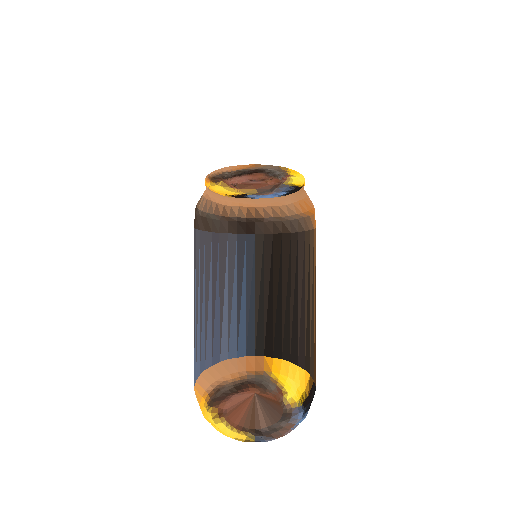
\includegraphics[width=0.5\textwidth]{flat_result.png}
    \caption{\gr Απόδοση του αντικειμένου με τεχνική \en Flat Shading\gr.}
\end{figure}

\begin{figure}[H]
    \centering
    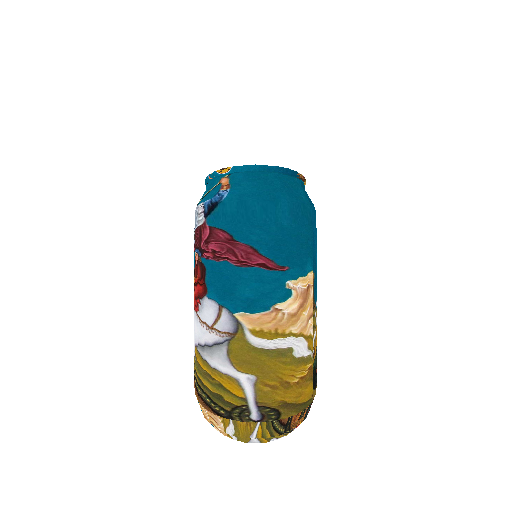
\includegraphics[width=0.5\textwidth]{texture_result.png}
    \caption{\gr Απόδοση του αντικειμένου με τεχνική \en Texture Mapping\gr.}
\end{figure}

\begin{figure}[H]
    \centering
    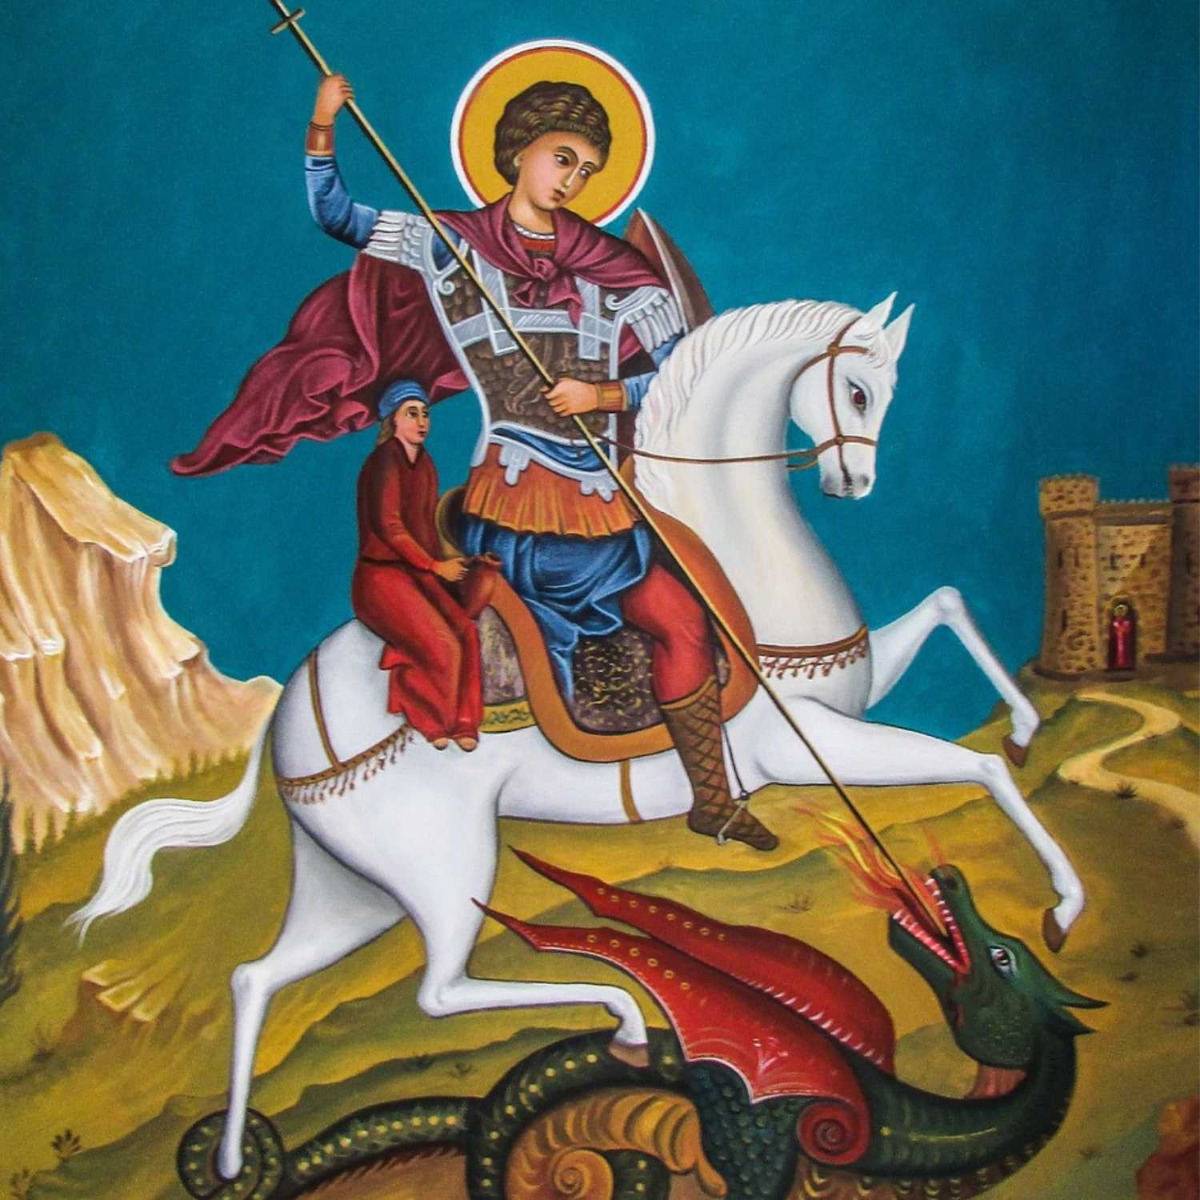
\includegraphics[width=0.5\textwidth]{texImg.jpg}
    \caption{\gr Εικόνα υφής που χρησιμοποιήθηκε για την τεχνική \en Texture Mapping\gr.}
\end{figure}

\section{Παρατηρήσεις}

\begin{itemize}
    \item Η τεχνική \en \textbf{Flat Shading} \gr είναι πιο απλή υπολογιστικά και οδηγεί σε ένα «μονοχρωματικό» αποτέλεσμα ανά τρίγωνο. Αυτό όμως προκαλεί μια απότομη μετάβαση χρωμάτων μεταξύ των τριγώνων, ειδικά σε περιοχές με έντονες μεταβολές στο χρώμα.
    
    \item Η τεχνική \en \textbf{Texture Mapping} \gr αποδίδει ένα πολύ πιο ρεαλιστικό αποτέλεσμα, καθώς η εικόνα υφής «τυλίγεται» γύρω από το αντικείμενο με βάση τις $UV$ συντεταγμένες. Το αποτέλεσμα εξαρτάται άμεσα από την ποιότητα και σωστή τοποθέτηση της υφής.
    
    \item Όπως φαίνεται στις παραπάνω εικόνες, η υφή με την εικόνα του Αγίου Γεωργίου εφαρμόζεται επιτυχώς επάνω στην κυλινδρική επιφάνεια του αντικειμένου, αποδεικνύοντας τη σωστή λειτουργία του αλγορίθμου.
    
    \item Σημαντικό ρόλο παίζει η \en \texttt{vector\_interp}\gr, η οποία εξασφαλίζει τη σωστή γραμμική παρεμβολή $UV$ συντεταγμένων κατά μήκος κάθε \en \texttt{scanline}\gr, έτσι ώστε κάθε \en \texttt{pixel} \gr να αντιστοιχεί σε σωστή θέση της εικόνας υφής.
\end{itemize}

\section{Συμπεράσματα}

Η υλοποίηση πέτυχε τους στόχους της, προσφέροντας δύο σαφώς διακριτές μεθόδους χρωματισμού. Η \en Flat Shading \gr προτείνεται για εφαρμογές με περιορισμένους πόρους, ενώ η \en Texture Mapping \gr είναι ιδανική για φωτορεαλιστική απόδοση γεωμετρικών μοντέλων. Η σωστή προετοιμασία των δεδομένων ($UV$, βάθος, κανονικοποίηση) είναι κρίσιμη για την επιτυχία κάθε τεχνικής.





\bibliographystyle{plain}
\begin{thebibliography}{1}
    \bibitem{lnmpikas}
    \en https://docs.opencv.org/4.x/d9/df8/tutorial\_root.html
\end{thebibliography}

\end{document}